\documentclass[compress]{beamer}
\usepackage[utf8]{inputenc}
\usepackage{default}
\usepackage[T1]{fontenc}
\usepackage[spanish]{babel}
\usepackage{graphicx}
\usepackage{subfigure}
\usepackage{wrapfig} %Figuras al lado de texto
\usepackage[rflt]{floatflt} %Figuras flotantes entre el texto
\usepackage{eso-pic}
\usepackage[absolute,overlay]{textpos}
\usepackage{calc}
\usepackage{tikz}
\usepackage{longtable,multirow,booktabs,titling}
\usepackage{tikz}
\usepackage{verbatim}
\usepackage{multimedia}
\usepackage{fontawesome}
  

\uselanguage{spanish}
\languagepath{spanish}
\deftranslation[to=spanish]{WHO?}{¿Quién?}
\deftranslation[to=spanish]{WHEN?}{¿Cuando?}
\definecolor{beamer@solarized@green}{HTML}{859900}
\usefonttheme{serif}
\setbeamercovered{transparent}
\usetheme{JuanLesPins}
\setbeamercolor{titlelike}{parent=structure} %%% Para quitarle el color de fondo
\usecolortheme[RGB={46,139,87}]{structure}
%\useoutertheme{shadow}
\useoutertheme[]{miniframes}
\useinnertheme{circles}
\usefonttheme[onlylarge]{structuresmallcapsserif}
\setbeamerfont{title}{shape=\itshape,family=\rmfamily}
\usetikzlibrary{positioning}
%\hspace{-3.5cm}
\title{\Large{Todo lo que necesitas saber para ser un ornitólogo \\ }}\\[1cm]
\author{
  \small{Dorantes Nieto Fernando} \\
  \small{Figueroa Álvarez Juan Andrés} \\
  \small{Jiménez Moreno Francisco Javier}}\\%[-2cm]
\date{19 de Agosto de 2017}
\usebackgroundtemplate { %
\includegraphics[ width=\paperwidth,height=\paperheight] {imagenes/fondo.png}}

\section{}
\begin{document}
\begin{frame}
\begin{wrapfigure}{c}{2cm}
%\includegraphics[width= 1cm]{imagenes/escudob.png}
\end{wrapfigure} 
% \begin{wrapfigure}{r}{0.5cm}
%   \includegraphics[width= 1.5cm]{imagenes/logotipoalasurbanas6.jpg}
% \end{wrapfigure}
\titlepage
\vspace{-1cm}
%\begin{enumerate}
 %\item \tiny{Tesis que para presentar título de biólogo}
% \item \tiny{Desarrollado con \LaTeX}
%\end{enumerate}
\end{frame}

\section{¿Qué es un ave?}
{
\usebackgroundtemplate{\includegraphics[width=\paperwidth,height=\paperheight]{imagenes/fondo2.png}}
  \begin{frame}
    \frametitle{¿Qué son las aves?}
    \vspace{-0.5cm}
    Las aves son organismos bastante interesantes..
    \begin{columns}[c]
      \column{.6\textwidth}
	  \visible<2,3>{
			\begin{center}
			  \includegraphics[scale=0.1]{imagenes/bird_anatomy-09_skeletal_system.png}\\
			   \captionof{}{Son Vertebrados.\textsuperscript{1}}
			\end{center}
			}
	\column{.6\textwidth}<3>
	   \visible<3,3>{
	   \begin{center}
	      \includegraphics[scale=0.2]{imagenes/plumas.jpg}\\
	      \captionof{}{Tienen plumas.\textsuperscript{2}}
	    \end{center}
	    }
      \end{columns} \\[1.5cm]

      \tiny{1 Tomado de: https://academy.allaboutbirds.org/all-about-bird-anatomy/}\\
      \tiny{2 Tomado de: https://es.pinterest.com/search/pins/?q=plumas }
      
 \end{frame}
}

{
\usebackgroundtemplate{\includegraphics[width=\paperwidth,height=\paperheight]{imagenes/fondo3.png}}
  \begin{frame}
    \frametitle{¿Qué son las aves?}
    \vspace{-0.5cm}
    Las aves también...
    \begin{columns}[c]
      \column{.6\textwidth}
	  \visible<2,3>{
			\begin{center}
			  \includegraphics[scale=0.31]{imagenes/pico.jpg}\\
			   \captionof{}{Tienen pico. \textsuperscript{1}}
			\end{center}
			}
	\column{.6\textwidth}<3>
	   \visible<3,3>{
	   \begin{center}
	      \includegraphics[scale=0.1]{imagenes/huevosAvesAlasUrbanas.jpg}\\
	      \captionof{}{Ponen huevos. \textsuperscript{2}}
	    \end{center}
	    }
      \end{columns} \\[1.5cm]

     \tiny{1 Tomado de: http://www.birdsleuth.org/beaks/}\\
     \tiny{2 Foto Rodrigo Alam González Alas Urbanas Club de Observadores}
 \end{frame}
}

{
\usebackgroundtemplate{\includegraphics[width=\paperwidth,height=\paperheight]{imagenes/fondo2.png}}
  \begin{frame}
    \frametitle{¿Qué otras características hacen a las aves únicas?}
    \vspace{-0.5cm}
    \begin{columns}[c]
      \column{.6\textwidth}
	  \visible<2,3>{
			\begin{center}
			  \includegraphics[scale=0.2]{imagenes/bird_anatomy-08_respiratory_system-764x537.png}\\
			  \captionof{}{Sistema respiratorio con sacos aéreos. \textsuperscript{1}}
			\end{center}
			}
	\column{.6\textwidth}<3>
	   \visible<3,3>{
	   \begin{center}
	      \includegraphics[scale=0.4]{imagenes/hueso_ave.jpg}\\
	      \captionof{}{Huesos `huecos'.\textsuperscript{2}}
	    \end{center}
	    }
      \end{columns} \\     
     \begin{center}
      Todo esto son características que definen a las aves.\\
     \end{center}
      
      \tiny{1 Tomado de: https://academy.allaboutbirds.org/all-about-bird-anatomy}\\
      \tiny{2 Tomado de: http://cmapspublic2.ihmc.us/rid=1M0BNBZXT-JQ2XRM-1R98/hueso_ave.jpg}

    
    
 \end{frame}
}

\section{Aves en el mundo y en México}
  
{
\usebackgroundtemplate{\includegraphics[width=\paperwidth,height=\paperheight]{imagenes/fondo3.png}}
  \begin{frame}
    \frametitle{¿Cuántas aves hay en el mundo?}
    
    \begin{enumerate}
     \item Se calcula que en el mundo existen entre 9000 y 9720 especies de aves.
     \item  México tiene alrededor de 1100 especies de aves (11\% del total mundial).
     \item Teniendo en cuenta el área  de México: 1,964,375 km2
     \item Y el área de todas las tierras emergidas: 148,940,000 km2
    \end{enumerate}       
    
    \begin{center}
     \textbf{¡En  1\% del territorio de tierras se encuentran 11 \% de especies de aves.!}\\
     ¿Por qué pasa esto?
    \end{center}

 \end{frame}
}

{
\usebackgroundtemplate{\includegraphics[width=\paperwidth,height=\paperheight]{imagenes/fondo2.png}}
  \begin{frame}
    \frametitle{Paises megadiversos}
    \begin{center}
      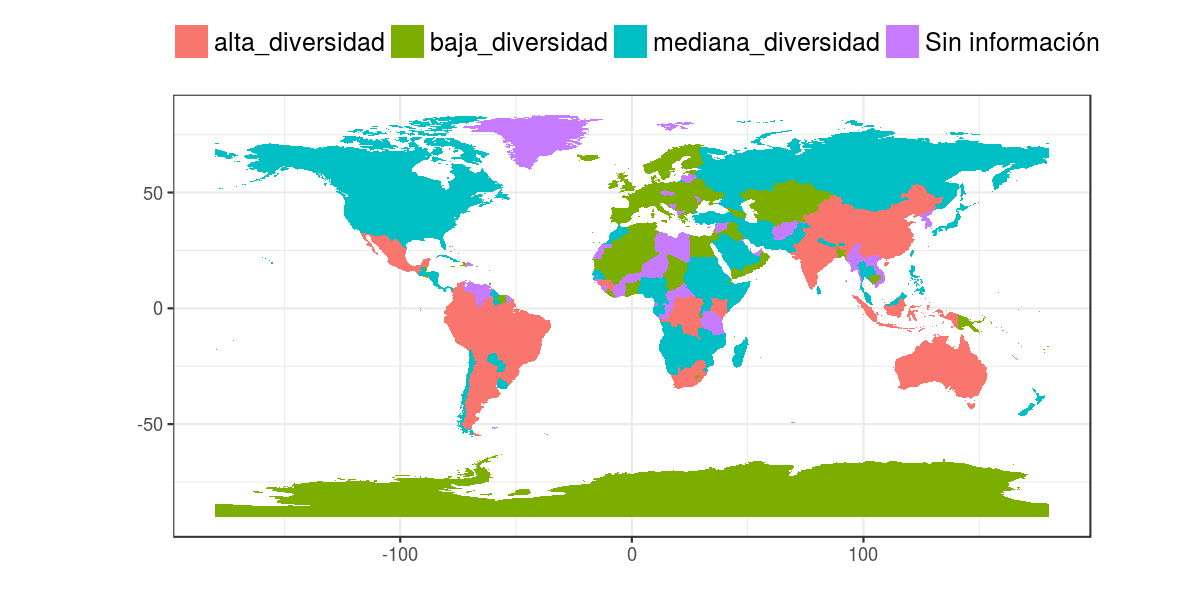
\includegraphics[scale=0.5]{graficos/mapaAves.png}\\
      \captionof{}{Diversidad de aves a nivel mundial.}
    \end{center}
    \tiny{Fuente: Checklist 2017, Cornell Lab Ornithology}\\
    \tiny{Gráfico: Fernando Dorantes}
 \end{frame}
}


{
\usebackgroundtemplate{\includegraphics[width=\paperwidth,height=\paperheight]{imagenes/fondo3.png}}
  \begin{frame}
    \frametitle{¿Qué pasa dentro de territorio mexicano?}
    \begin{center}
      Los primeros diez estados con más especies en México: \\[0.2cm]
      {\tiny
	\begin{tabular}{ccc} \toprule
	  Estado & Fuente & Número de especies \\ \midrule
	  Oaxaca & Binfor (1989) & 699 \\[0.2cm]
	  Veracruz & Alcántara (en proceso) & 687 \\ [0.2cm]
	  Chiapas & Álvarez del Toro (1980) & 647 \\ [0.2cm]
	  \textbf{Puebla} & Rojas(1995)/\textbf{Aves del estado de Puebla} (2014) & 481/ \textbf{599} \\ [0.2cm]
	  Guerrero & Navarro Benitez (en proceso) & 523 \\ [0.2cm]
	  Sonora & Van Rossem (1945) & 431 \\ [0.2cm]
	  Nayarit & Escalante (1988) & 409 \\ [0.2cm]
	  Colima & Schaldach (1963) & 365 \\ [0.2cm]
	  Yucatán & Paynter (1955) & 356 \\ [0.2cm]
	  Baja California & Grinnel (1928) Wilbur(1987) & 353 \\ \hline
	  \end{tabular}}
    \end{center}\\[0.2cm]
    
    \tiny(Fuente: (Castán et al, 2014, Aves del estado de Puebla))

 \end{frame}
}

{
\usebackgroundtemplate{\includegraphics[width=\paperwidth,height=\paperheight]{imagenes/fondo2.png}}
  \begin{frame}
    \frametitle{Aves en el estado de  Puebla}
    \begin{center}
      Puebla tiene 599 especies de aves de las 1100 que existen en el país.\\
      Eso significa el 54\% de las especies.\\
      En resumen el estado de Puebla tiene...\\
    \end{center}
    \begin{enumerate}
     \item 19 órdenes de especies de aves.\\ [0.2cm]
     \item 67 familias.\\ [0.2cm]
     \item 309 géneros. \\ [0.2cm]
    \end{enumerate} \\[0.2cm]
    
    \tiny(Fuente: (Castán et al, 2014, Aves del estado de Puebla))
 \end{frame}
}

{
\usebackgroundtemplate{\includegraphics[width=\paperwidth,height=\paperheight]{imagenes/fondo3.png}}
  \begin{frame}
    \frametitle{Aves en el estado de  Puebla}
    \begin{center}
      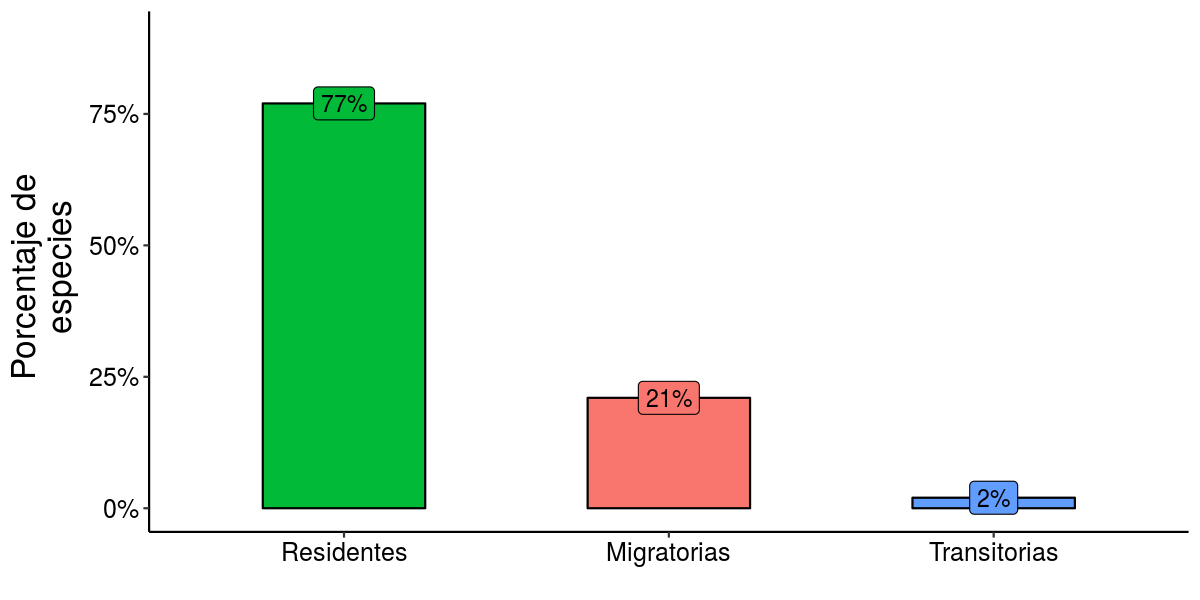
\includegraphics[scale=0.5]{graficos/porcentajeAvesPuebla.png}\\
      \captionof{}{Porcentaje de especies de aves en Puebla por estacionalidad.}
    \end{center}

 \end{frame}
}


{
\usebackgroundtemplate{\includegraphics[width=\paperwidth,height=\paperheight]{imagenes/fondo3.png}}
  \begin{frame}
    \frametitle{Aves en la ciudad  Puebla}
    \begin{center}
      Se tienen registradas 241 especies en la ciudad de Puebla (Zona urbana y alrededores).\\
      En otros rangos taxonómicos esto significa:\\
      \begin{enumerate}
       \item 20 órdenes
       \item 51 familias
      \end{enumerate}
      Con respecto a estacionalidad: \\
      \begin{enumerate}
       \item 101 especies migratorias
       \item 141 especies residentes
      \end{enumerate}
      
    \end{center} \\[0.2cm]

     \tiny(Fuente: (Mendoza-Cuamatzi et al, 2012, Las aves del municipio de Puebla))


 \end{frame}
}

\section{Observando aves}
{
\usebackgroundtemplate{\includegraphics[width=\paperwidth,height=\paperheight]{imagenes/fondo2.png}}
  \begin{frame}
    \frametitle{}
    \begin{center}
      \textbf{
      Con tantas especies en México y el mundo.
      El observar aves implica conocer un poco de toda esa biodiversidad.}
    \end{center}
         
     \begin{center}
      \includegraphics[scale=0.3]{imagenes/caricatura1.jpg}\\
      \captionof{}{}
    \end{center}



 \end{frame}
}


{
\usebackgroundtemplate{\includegraphics[width=\paperwidth,height=\paperheight]{imagenes/fondo2.png}}
  \begin{frame}
    \frametitle{Algunos consejos antes de iniciar}
    Cuando usted observe aves....
    \begin{itemize}
    \pause
     \item Siempre ser respetuoso y no incomodar a las personas a 
	   tu alrededor que no estén observando aves.
      \pause
     \item Siempre respetar propiedad privada. 
	   \textbf {A pesar de que el registro sea muy raro.}
      \pause
     \item No vestir con colores muy vistosos. ¡Las aves se asustan más fácil!
     \pause
     \item Caminar lento. El ir rápido puede asustar a las aves.
    \end{itemize}
 \end{frame}
}


{
\usebackgroundtemplate{\includegraphics[width=\paperwidth,height=\paperheight]{imagenes/fondo3.png}}
  \begin{frame}
    \frametitle{¿Qué necesito para observar aves?}
    \begin{center}
      \includegraphics[scale=0.2]{imagenes/observarAves2.png}\\
      \captionof{}{}
    \end{center}

    \tiny{Fuente: Museo de las aves de México}
   
 \end{frame}
}

{
\usebackgroundtemplate{\includegraphics[width=\paperwidth,height=\paperheight]{imagenes/fondo2.png}}
  \begin{frame}
    \frametitle{El binocular}
    Los conocemos como binoculares pero según la RAE \textsuperscript{1} la
    palabra correcta para designar a este instrumento es: El binocular.
    
    Existen dos tipos:
    \begin{columns}[c]
      \column{.6\textwidth}
	  \visible<2,3>{
			\begin{center}
			  \includegraphics[scale=0.2]{imagenes/techoBinocularUnion.png}\\
			   \captionof{}{Tipo Techo.\textsuperscript{2}}
			\end{center}
			}
	\column{.6\textwidth}<3>
	   \visible<3,3>{
	   \begin{center}
	      \includegraphics[scale=0.2]{imagenes/porroBinocularUnion.png}\\
	      \captionof{}{Tipo Porro.\textsuperscript{2}}
	    \end{center}
	    }
      \end{columns} \\[1.5cm]
    
    \tiny{1 Fuente: http://dle.rae.es/srv/search?m=30&w=binocular}\\
    \tiny{2 Fuente: www.astroshop.es}
 \end{frame}
}


{
\usebackgroundtemplate{\includegraphics[width=\paperwidth,height=\paperheight]{imagenes/fondo3.png}}
  \begin{frame}
    \frametitle{El binocular}
    \begin{center}
      \includegraphics[scale=0.1]{imagenes/eleccionBinocular1.png}\\
      \captionof{}{}
    \end{center}

   
 \end{frame}
}

{
\usebackgroundtemplate{\includegraphics[width=\paperwidth,height=\paperheight]{imagenes/fondo2.png}}
  \begin{frame}
    \frametitle{Identificando aves}
    \framesubtitle{La forma}
    \begin{center}
      \includegraphics[scale=0.4]{imagenes/silhouettes-sceneFondoNo.png}\\
      \captionof{}{}
    \end{center}\\[-0.2cm]

   \tiny{Tomado de : http://www.birdsleuth.org/teaching-bird-id/}
 \end{frame}
}


{
\usebackgroundtemplate{\includegraphics[width=\paperwidth,height=\paperheight]{imagenes/fondo3.png}}
  \begin{frame}
    \frametitle{Identificando aves}
    \framesubtitle{El pico}
    \begin{center}
      \includegraphics[scale=0.3]{imagenes/beaks.png}\\
      \captionof{}{}
    \end{center}\\[-0.2cm]

   \tiny{Tomado de : https://www.researchgate.net/figure/308946274_fig1_Fig-1-Diversity-in-size-and-shape-of-beaks-underlies-their-role-in-resource}
 \end{frame}
}

{
\usebackgroundtemplate{\includegraphics[width=\paperwidth,height=\paperheight]{imagenes/fondo2.png}}
  \begin{frame}
    \frametitle{Identificando aves}
    \framesubtitle{El tamaño}
    \begin{center}
      \includegraphics[scale=0.4]{imagenes/tamanioModificado.jpg}\\
      \captionof{}{}
    \end{center}\\[-0.2cm]

   \tiny{Tomado con modificaciones : http://www.spokesman.com/blogs/outdoors/2014/feb/03/shape-your-birding-knowledge-chart/}
   \end{frame}
}

{
\usebackgroundtemplate{\includegraphics[width=\paperwidth,height=\paperheight]{imagenes/fondo3.png}}
  \begin{frame}
    \frametitle{Identificando aves}
    \framesubtitle{La forma de vuelo}
    \begin{center}
      \includegraphics[scale=0.25]{imagenes/colibriMarcoAlasUrbanas.jpg}\\
      \captionof{}{}
    \end{center}\\[-0.2cm]

   \tiny{Foto: Marco Arturo Vidal Bolaños Alas urbanas club de Observadores }
   \end{frame}
}

{
\usebackgroundtemplate{\includegraphics[width=\paperwidth,height=\paperheight]{imagenes/fondo2.png}}
  \begin{frame}
    \frametitle{Identificando aves}
    \framesubtitle{Donde viven, que comen y como se comportan.}
    \begin{center}
      \includegraphics[scale=0.12]{imagenes/collage1.png}\\
      \captionof{}{}
    \end{center}\\[-0.2cm]

   \tiny{Foto: Autores varios, Alas urbanas club de Observadores }
   \end{frame}
}

{
\usebackgroundtemplate{\includegraphics[width=\paperwidth,height=\paperheight]{imagenes/fondo3.png}}
  \begin{frame}
    \frametitle{Identificando aves}
    \framesubtitle{El canto.}
    \begin{center}
      \includegraphics[scale=0.2]{imagenes/cantos.png}\\
      \captionof{}{}
    \end{center}\\[2cm]    
        
   \tiny{Tomado de http://songbirdscience.com/}
   \end{frame}
}

{
\usebackgroundtemplate{\includegraphics[width=\paperwidth,height=\paperheight]{imagenes/fondo2.png}}
  \begin{frame}
    \frametitle{Identificando aves}
    \framesubtitle{El canto.}
    \begin{center}
	Ejemplos de cantos...
      \begin{columns}[c]
      \column{.6\textwidth}
	  \visible<2,3>{
			\begin{center}
			  \includegraphics[scale=0.1]{imagenes/coquitaMarcoArturo.jpg}\\
			   \captionof{Tortola Coquita \textsuperscript{1}\\}{
			       \sound[autostart,inlinesound]{
				\hyperlink{columns}{\beamergotobutton{{\textit{Columbina Inca}}}}
				      }{columbinaInca.mp3}\\

			   }
			\end{center}
			}
	\column{.6\textwidth}<3>
	   \visible<3,3>{
			\begin{center}
			  \includegraphics[scale=0.22]{imagenes/dives_dives.jpg}\\
			   \captionof{Tordo Cantor \textsuperscript{2}\\}{
			      \sound[autostart,inlinesound]{
				  \hyperlink{columns}{\beamergotobutton{{\textit{Dives dives}}}}
				 }{divesDives.mp3}\\

			  }
			\end{center}
		    }
      \end{columns} \\[1.5cm]

    \end{center}
        
   \tiny{1 Foto: Marco Arturo Vidal Bolaños Alas Urbanas Club de Observadores}\\
   \tiny{2 Foto: Andy Jones Naturalista http://www.naturalista.mx/photos/67526}
   \end{frame}
}




{
\usebackgroundtemplate{\includegraphics[width=\paperwidth,height=\paperheight]{imagenes/fondo2.png}}
  \begin{frame}
    \frametitle{Guías de identificación}
    \framesubtitle{¿Qué usar para identificar?}
    \begin{center}
      \includegraphics[scale=0.12]{imagenes/guias.png}\\
      \captionof{}{}
    \end{center}\\[-0.2cm]

   %\tiny{Foto: Autores varios, Alas urbanas club de Observadores }
   \end{frame}
}

{
\usebackgroundtemplate{\includegraphics[width=\paperwidth,height=\paperheight]{imagenes/fondo3.png}}
  \begin{frame}
    \frametitle{Registrando mis observaciones}
    \framesubtitle{¿Donde guardo mis registros?}
    \begin{center}
      \includegraphics[scale=0.12]{imagenes/collageEbird1.png}\\
      \captionof{}{}
    \end{center}\\[-0.2cm]

   %\tiny{Foto: Autores varios, Alas urbanas club de Observadores }
   \end{frame}
}


{
\usebackgroundtemplate{\includegraphics[width=\paperwidth,height=\paperheight]{imagenes/fondo2.png}}
  \begin{frame}
    \frametitle{Registrando mis observaciones}
    \framesubtitle{¿Donde guardo mis registros?}
    \begin{center}
      \includegraphics[scale=0.12]{imagenes/collageEbird2.png}\\
      \captionof{}{}
    \end{center}\\[-0.2cm]

   %\tiny{Foto: Autores varios, Alas urbanas club de Observadores }
   \end{frame}
}




{
\usebackgroundtemplate{\includegraphics[width=\paperwidth,height=\paperheight]{imagenes/fondo3.png}}
  \begin{frame}
    \frametitle{Eventos de aves}
    \begin{center}
      \includegraphics[scale=0.12]{imagenes/collageEventos.png}\\
      \captionof{}{}
    \end{center}\\[-0.2cm]

   %\tiny{Foto: Autores varios, Alas urbanas club de Observadores }
   \end{frame}
}


\section{Conservación de las aves}

{
\usebackgroundtemplate{\includegraphics[width=\paperwidth,height=\paperheight]{imagenes/fondo3.png}}
  \begin{frame}
    \frametitle{}
    \textbf{
      Si bien convivimos este planeta con millones de organismos.
      No todos están a salvo.
      Las aves no son la excepción...}
   \end{frame}
}

{
\usebackgroundtemplate{\includegraphics[width=\paperwidth,height=\paperheight]{imagenes/fondo2.png}}
  \begin{frame}
    \frametitle{Extinción de aves}
      \begin{center}
	\includegraphics[scale=0.25]{imagenes/extincion.jpg}\\
	\captionof{}{}
      \end{center}\\[-0.2cm]

   \tiny{Fuente: https://conabio.gob.mx }   \end{frame}
}


{
\usebackgroundtemplate{\includegraphics[width=\paperwidth,height=\paperheight]{imagenes/fondo2.png}}
  \begin{frame}
    \frametitle{Causas de pérdida de biodiversidad mundial}
    
      \begin{center}
	\LARGE EL ANTROPOCENO \\[0.2CM]
	\includegraphics[scale=0.3]{imagenes/ciudad.jpg}\\
	\captionof{}{}
      \end{center}\\[-0.2cm]

   \tiny{Imágen: http://www.huffingtonpost.es/2013/01/11/central-park-desde-el-aire_n_2455837.html }  
   \end{frame}
}

{
\usebackgroundtemplate{\includegraphics[width=\paperwidth,height=\paperheight]{imagenes/fondo3.png}}
  \begin{frame}
    \frametitle{Causas de pérdida de biodiversidad mundial}
    
      \begin{center}
	\LARGE CAMBIO CLIMÁTICO \\[0.2CM]
	\includegraphics[scale=0.3]{imagenes/cambioclimatico.jpg}\\
	\captionof{}{}
      \end{center}\\[-0.2cm]

   \tiny{Imágen: http://geo-mexico.com/?p=3216 }  
   \end{frame}
}

{
\usebackgroundtemplate{\includegraphics[width=\paperwidth,height=\paperheight]{imagenes/fondo3.png}}
  \begin{frame}
    \frametitle{Causas de pérdida de biodiversidad mundial}
    
      \begin{center}
	\includegraphics[scale=0.15]{imagenes/collage2.png}\\
	\captionof{}{}
      \end{center}\\[-0.2cm]

   \tiny{Imágen: http://geo-mexico.com/?p=3216 }  
   \end{frame}
}

{
\usebackgroundtemplate{\includegraphics[width=\paperwidth,height=\paperheight]{imagenes/fondo2.png}}
  \begin{frame}
    \frametitle{Conservación de aves}
      Sin embargo, hay muchas personas que estudian a las aves.
      Crean estrategias de conservación y ayudan a preservar esta biodiversidad.
      
      No obstante nosotros también podemos ayudar a 
      conservar a las aves....

   \end{frame}
}


{
\usebackgroundtemplate{\includegraphics[width=\paperwidth,height=\paperheight]{imagenes/fondo3.png}}
  \begin{frame}
    \frametitle{}
      \begin{center}
	  \LARGE GRACIAS POR SU ATENCIÓN
      \end{center}
      \begin{center}
	\includegraphics[scale=0.2]{imagenes/tortolitasMarcoAlas.jpg}\\
	\captionof{}{}
      \end{center}\\[-0.2cm]

   \tiny{Foto: Marco Arturo Vidal Bolaños Alas Urbanas Club de Observadores }  
 
    

   \end{frame}
}

{
\usebackgroundtemplate{\includegraphics[width=\paperwidth,height=\paperheight]{imagenes/fondo3.png}}
  \begin{frame}
    \frametitle{}
      \begin{center}
	  \LARGE ¿PREGUNTAS?
      \end{center}
      \begin{center}
	\includegraphics[scale=0.4]{imagenes/dinosaurs.jpg}\\
	\captionof{}{}
      \end{center}\\[-0.2cm]

 
    

   \end{frame}
}


\end{document}

